\documentclass[aspectratio=169]{beamer}

\usetheme{Starkville}

\title{An Example Presentation}
\author{Dakota Hester}
\institute{Mississippi State University \\ Department of Agricultural and Biological Engineering}
\date{\today}

\logo{
\includegraphics[height=4.75\baselineskip]{images/ABE_Logo_Vertical_White.png}}

\begin{document}

\begin{frame}{Name of Conference, Event, Course, etc.}
    \titlepage
    \centering
    
\includegraphics[width=2.5cm]{images/gcerlogo.png}
\end{frame}

\begin{frame}{Overview}
    \tableofcontents
\end{frame}

\section{Introduction}
\begin{frame}{Introduction}
    \begin{itemize}
        \item This is the first item
        \item This is the second item
        \item This is the third item
    \end{itemize}
\end{frame}

\section{Background}

\subsection{Prior Work}
\begin{frame}{Einsten et al.}
    \begin{enumerate}
        \item First
        \item Second
        \item Third
    \end{enumerate}
\end{frame}

\section{Methods}

\subsection{Data Collection}
\begin{frame}{Methods}
    \alert{This is an alert} and this is not.
\end{frame}

\begin{frame}{Hail State}
    \begin{block}{Block Title}
        This is a block.
    \end{block}
    \begin{alertblock}{Alert Block Title}
        This is an alert block.
    \end{alertblock}
    \begin{exampleblock}{Example Block Title}
        This is an example block.
    \end{exampleblock}
\end{frame}

\section{Results}

\begin{frame}{Baseball Scores}
    \begin{table}
        \centering
        \begin{tabular}{c|c}
            \hline
            A & B \\
            \hline
            1 & 2 \\
            3 & 4 \\
            5 & 6 \\
            \hline
        \end{tabular}
        \caption{This is a table full of interesting data.}
    \end{table}
\end{frame}

\section{Discussion}

\begin{frame}{Interesting Figure}
    \begin{figure}
        \centering
        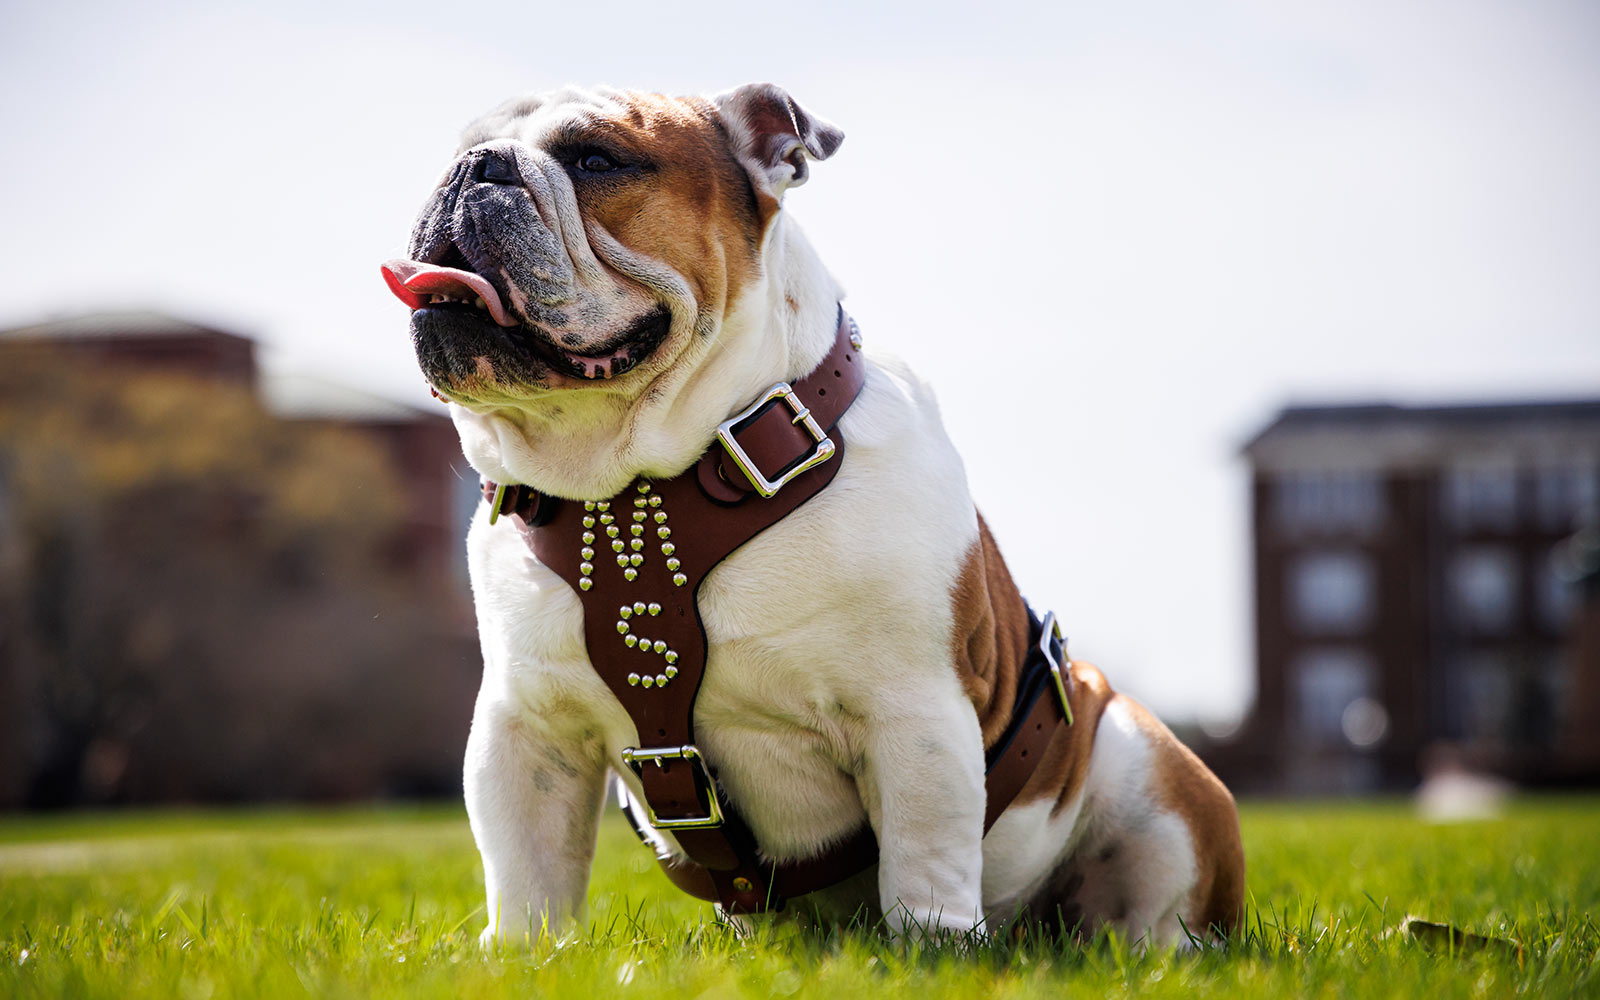
\includegraphics[width=0.5\textwidth]{images/bully.jpg}
        \caption{This is a figure.}
    \end{figure}
\end{frame}

\section{Conclusion}

\begin{frame}{Conclusion}
    \begin{columns}
        \begin{column}{0.5\textwidth}
            This is a column.
        \end{column}
        \begin{column}{0.5\textwidth}
            \begin{center}
                \alert{Acknowledgements}
                \begin{itemize}
                    \item Hey look!
                    \item Another list!
                    \begin{itemize}
                        \item With subitems!
                        \item And more subitems!
                        \item And even more subitems!
                    \end{itemize}
                \end{itemize}
            \end{center}
        \end{column}
    \end{columns}
\end{frame}

\end{document}